\documentclass[10pt]{article}

\usepackage[utf8]{inputenc}
\usepackage[T1]{fontenc}
\usepackage[margin=1in]{geometry}
\usepackage{authblk}
\usepackage{graphicx}
\usepackage{booktabs}
\usepackage{array}
\usepackage{longtable}
\usepackage[protrusion=true,expansion=false]{microtype}
\usepackage{xcolor}
\usepackage{amsmath}
\usepackage[numbers,super,sort&compress]{natbib}
\usepackage{url}
\usepackage{seqsplit}
\usepackage{xspace}
\usepackage[hidelinks]{hyperref}
\usepackage{cleveref}
\usepackage{placeins}

\setlength{\emergencystretch}{3em}
\Urlmuskip=0mu plus 1mu

\renewcommand{\Authfont}{\large\bfseries}
\renewcommand{\Affilfont}{\small\normalfont}
\setlength{\affilsep}{0.5em}

\graphicspath{{figures/generated/}}
\newcommand{\dataset}{\textsc{PT60-Candidate}\xspace}
\newcommand{\project}{\textsc{PortugueseOPD}\xspace}
\newcommand{\code}[1]{\texttt{#1}}
\newcommand{\hashvalue}[1]{\texttt{\seqsplit{#1}}}
\newcommand{\status}[1]{\textsc{#1}}
\newcommand{\osmevidence}{OSM-derived public evidence\xspace}
\newcommand{\doi}[1]{\url{https://doi.org/#1}}

\title{A provenance-tracked candidate dataset for Portuguese 60~kV topology reconstruction}
\author[1]{Author details to be finalized before submission}
\affil[1]{Affiliation details to be finalized before submission}
\date{July 2026}

\begin{document}
\maketitle

\begin{abstract}
Public distribution-network records rarely provide explicit bus--branch topology, limiting their direct reuse for power-grid modelling and geospatial network analysis. We present \dataset, a provenance-tracked candidate dataset for the Portuguese E-REDES 60~kV network layer, built with a fail-closed pipeline that preserves unresolved or ambiguous records with blocking reasons rather than silently promoting them. From 5,334 line features and 586 facility records, the selected configuration produces 1,341 classified circuit candidates: 358 retained inter-facility branches and 983 downgraded or rejected records (hereafter non-retained outcomes) with documented reasons. \dataset{} includes a 484-node multigraph, a 216-configuration sensitivity sweep, source manifests, machine-readable schemas, a field-level data dictionary, checksums, and branch-level public-evidence records derived from OpenStreetMap (OSM). Internal validation checks geometry, identifiers, graph--table parity, schema coverage, missingness, and archive integrity. Endpoint-name permutation and displaced-geometry controls reduce the corresponding OSM-evidence rates by 95.1\% and 99.7\%, supporting matcher selectivity. \dataset{} provides a reusable data foundation for topology-reconstruction research, provenance-aware power-network analysis, geospatial integration, sensitivity assessment, and the development of graph and tabular data interfaces. Versioned data and code are publicly available.
\end{abstract}

\noindent\textbf{Keywords:} power-grid dataset; open power-grid data; data provenance; topology reconstruction; distribution networks; geospatial network analysis; technical validation

\section{Background \& Summary}

Public distribution-network portals can support open power-grid research, geospatial network analysis, and data-driven modelling, but the released records rarely correspond directly to an auditable bus--branch dataset. Connectivity must usually be inferred from facility locations and line geometries, while electrical parameters, switching states, and operating conditions may remain incomplete or unavailable. In this setting, a reusable dataset should not only provide candidate connections; it should also preserve how those candidates were constructed, what evidence supports them, and which fields remain unknown, inferred, or diagnostic.

\dataset was assembled to provide such a resource for the Portuguese E-REDES 60~kV network layer. It converts public geospatial records into a provenance-tracked candidate topology dataset, with retained branches, non-retained circuit outcomes, validation outputs, release manifests, and downstream interface contracts kept inspectable as part of the data record. The aim is to provide a reusable data foundation for topology-reconstruction research, provenance-aware power-network analysis, geospatial integration, sensitivity assessment, and future digital modelling of distribution-network data.

The release contains three closely related resource types. First, it provides a core topology layer composed of retained inter-facility branches, an all-facility multigraph, and a complete circuit-classification ledger. Second, it provides validation and provenance records, including a reconstruction-sensitivity sweep, a source manifest, public-source audits, negative controls, and branch-level triangulation outputs. Third, it provides a schema package, field-level data dictionary, join documentation, manifest, checksums, and responsible-use metadata so that the core records can be interpreted and reused without depending on the development repository.

The contribution is a documented, reusable, and provenance-tracked data resource for studying how public grid records can be converted into inspectable graph and tabular representations. European open-grid resources demonstrate the reuse value of transparent model construction and standardized public records \cite{Medjroubi2017,Horsch2018,Wiese2019,Xiong2025}; OSM-based reconstruction studies also show that public geometry requires explicit topology-building assumptions \cite{Rivera2019,Haklay2008}. Dataset documentation and FAIR practice motivate the release of provenance, field semantics, identifiers, and reuse constraints alongside the data \cite{Wilkinson2016,Gebru2021}. \dataset applies these principles to a Portuguese 60~kV distribution-layer reconstruction while exposing retained branches, non-retained outcomes, semantic status fields, and validation evidence in machine-readable form.

\section{Methods}

\subsection{Source datasets}

The source snapshot combines AT line geometries, AT substations, switching facilities, MT-substation context, network-characteristics tables, substation-load records, reception-capacity context, and load-diagram indices from the E-REDES Open Data Portal \cite{EREDESOpenData2026}. Table~\ref{tab:source-inputs} identifies the three topology-critical inputs; the 13-source inventory and exact catalog, portal, CSV, and GeoJSON URLs are preserved in \code{provenance/reproduction\_source\_manifest.json}. For example, the line metadata route is \url{https://e-redes.opendatasoft.com/api/explore/v2.1/catalog/datasets/rede-at-teste}; the other routes substitute the identifiers shown in the table. The official RND page publicly embeds the widget API keys required by these layers. Metadata, record, and export requests returned HTTP~200 for all three topology-critical datasets at the reported access dates.

\begin{table}[t]
\centering
\small
\caption{Topology-critical E-REDES inputs. Record counts and keyed access checks are frozen provenance values from 13 July 2026. The required API keys are publicly discoverable from the official RND page widgets.}
\label{tab:source-inputs}
\begin{tabular}{p{0.20\textwidth}rp{0.14\textwidth}p{0.25\textwidth}p{0.11\textwidth}}
\toprule
Portal identifier & Records & Snapshot date & Role & Keyed access \\
\midrule
\code{rede-at-teste} & 5,334 & 2026-07-13 & AT line geometries & HTTP 200 \\
\code{se-at\_2025} & 410 & 2026-07-13 & AT substation facilities & HTTP 200 \\
\code{pc-at\_2025} & 76 & 2026-07-13 & Switching facilities & HTTP 200 \\
\bottomrule
\end{tabular}
\end{table}

The counts in Table~\ref{tab:source-inputs} precede exact-record deduplication. All 410 substation geometries are valid points, but source feature 372 duplicates feature 90 under the loader key (facility type, code, and coordinates; both are the LAGOA record with code \code{0806S5060700}); retaining the first occurrence leaves 409 AT substations. All 76 switching-facility geometries are likewise valid points, but feature 65 duplicates feature 14 under the same key (the LAMEIRAS record with code \code{0806P5061500}); retaining the first leaves 75 switching facilities. Node set B therefore contains $409+75=484$ facilities. With the 102 MT-context facilities, the topology stage loads 586 technically relevant facilities in total. It also loads 5,334 valid AT line features: 5,323 labelled 60~kV and 11 labelled 130~kV. The 11 130~kV features merge into five candidates (three self-loops, one single-facility record, and one isolated record). All five remain in the classification ledger; none enters the 358 retained branches, and no mixed-voltage circuit is produced.

The release uses the portal-level license statement reported by E-REDES for distributable data artifacts. The dataset package records publisher attribution, portal URL, source dataset identifiers, access dates, and transformation notices separately from the repository's MIT code license. Where topology-critical API catalog responses did not repeat an explicit license field, the release policy follows the recorded portal-level statement rather than inferring a different license from the omission. The topology-critical catalog records were checked on 13 July 2026; per-source timestamps are preserved in \code{provenance/reproduction\_source\_manifest.json}.

\subsection{Data acquisition}

Source files were acquired from the official E-REDES Open Data portal through the public API routes in Table~\ref{tab:source-inputs}. The manifest-driven workflow reads the official RND page to identify dataset identifiers and API keys, then requests metadata, records, and CSV or GeoJSON exports. Each response is logged with its route, access timestamp, HTTP status, record count, byte size, and SHA-256 digest. Geometry and schema checks precede reconstruction; acquisition or parsing failures stop the pipeline.

\subsection{Data preprocessing}

Preprocessing harmonizes source geometries, facility identifiers, and facility classes before topology inference. Released geometries use WGS84 longitude--latitude coordinates (EPSG:4326). The reconstruction workflow projects them to ETRS89 / Portugal TM06 (EPSG:3763), a metre-based projected coordinate reference system for mainland Portugal, for facility buffering, endpoint clustering, matching, corridor distances, and length calculations. Coordinates are transformed back to EPSG:4326 for released GeoJSON geometries. These transformations and geometry-derived quantities are recorded as derived rather than observed values. The comparison with the legacy local equirectangular implementation is reported under Technical Validation.

Facilities are standardized into node candidates with associated codes, names, types, source roles, and footprint-ready geometries. Source line features are standardized into endpoint-bearing line records. Ambiguous matches and unresolved endpoints are retained as explicit states for later classification. This preprocessing stage therefore prepares line and facility inputs for reconstruction without asserting that each input line already corresponds to a valid inter-facility branch.

\subsection{Provenance model}

The release uses a field-level semantic status model so that downstream users can separate copied observations from deterministic derivations, inferred topology, and diagnostic assumptions. For an object $o$ at stage $k$, the workflow records
\begin{equation}
T_k(o)=(v,s,q,a,e),
\end{equation}
where $v$ is the value, $s$ its semantic status, $q$ a quality or confidence indicator, $a$ a source or assumption identifier, and $e$ an exclusion or blocking reason.

\begin{table}[t]
\centering
\small
\caption{Semantic statuses used in \dataset and its derivative interfaces.}
\label{tab:semantics}
\begin{tabular}{p{0.19\textwidth}p{0.71\textwidth}}
\toprule
Status & Interpretation \\
\midrule
Observed & Copied from an E-REDES record, subject to source and join quality. \\
Derived & Deterministic transformation, such as geometry length. \\
Inferred & Connectivity produced by matching, clustering, merging, or classification. \\
Source-backed & Supported by an applicable operator, standard, or catalog source. \\
Scenario-assumed & Explicit choice used only in a named diagnostic scenario. \\
Benchmark-only & Non-Portuguese reference value used only for software and interface testing. \\
Proxy & Surrogate identity, injection, capacity, dispatch, or cost semantics. \\
Missing & Intentionally unfilled; dependent readiness gates must block use. \\
\bottomrule
\end{tabular}
\end{table}

Table~\ref{tab:semantics} summarizes the evidence distinctions carried into the released records and metadata so that consumers can apply explicit admissibility rules. The complete field-level dictionary is provided as \code{schema/data\_dictionary.csv}; \code{schema/file\_schema\_summary.csv}, \code{schema/join\_relationships.csv}, and \code{manifest.json} provide file-level structure, joins, versions, roles, and checksums.

\subsection{Reconstruction pipeline}

Facility records are converted to circular footprints with radii of 50, 100, 250, and 500~m. Three node sets are evaluated: set A contains 409 AT substations, set B contains 484 AT substations and switching facilities, and set C contains all 586 technically relevant facilities. Each source line contributes two endpoints. When an endpoint intersects multiple footprints, the workflow resolves membership by centroid distance and records ambiguity where needed rather than forcing an unqualified assignment.

Endpoints are then clustered at 0.5, 1, 5, 10, 25, and 50~m. Union--find merging groups features into circuit candidates under geometry-only, voltage-aware, or voltage-plus-status-aware compatibility rules. Explicit conflicts block merging in the corresponding compatibility mode. Endpoint-cluster degree is then used to distinguish ordinary terminal pairs from loop, self-loop, isolated, and tap or multi-terminal patterns.

Figure~\ref{fig:pipeline} shows how retained and non-retained outcomes pass through common validation and release-contract stages.

\begin{figure}[t]
  \centering
  
\includegraphics[width=\textwidth]{fig1_pipeline_overview.pdf}
  \caption{Fail-closed reconstruction and release workflow for \dataset. The 216-setting sweep and documented selection rule precede the selected configuration and declared inter-facility retention gate. Pass and fail-closed paths preserve retained and non-retained outcomes separately before common validation and packaging. OSM-derived public evidence enters only the validation stage. Counts are read from the frozen release and summarize dataset construction and internal checks.}
  \label{fig:pipeline}
\end{figure}

\subsection{Candidate selection}

A merged group is retained as an inter-facility candidate branch only when it has exactly two terminals, both terminals match facilities without disqualifying ambiguity, and the two facilities are distinct. Outcomes failing these conditions remain available in the circuit-classification ledger as non-retained loop, self-loop, single-facility, isolated, tap or multi-terminal, or ambiguous records.

This selection policy is intentionally conservative. It favors explicit preservation of non-retained outcomes over optimistic retention. Mixed voltage or status conflicts, suspicious spatial matches, and unresolved facility mappings are retained as audit information instead of being absorbed into a simplified final graph.

For each retained branch, the archived rule-based endpoint-proximity \code{confidence\_score} is
\begin{equation}
q=\max\!\left(0,\min\!\left(1,1-0.35\frac{d_{\max}}{b}\right)\right),
\end{equation}
where $d_{\max}$ is the larger of the two endpoint-to-facility distances and $b$ is the facility-buffer radius, both in metres. For retained branches, $0\leq d_{\max}/b\leq1$; the theoretical score range is therefore $[0.65,1.00]$, and the observed release range is 0.6529--0.9692. The factor 0.35 is a fixed scaling convention that preserves this range for retained matches and is rounded to four decimals. The field is a deterministic proximity score rather than a calibrated probability. It is computed only after a circuit passes the inter-facility retention rule and does not affect merging, retention, the 216-setting selection score, or the OSM-derived evidence category.

\subsection{Parameter sweep}

The reconstruction workflow evaluates 216 settings generated by combining three facility sets, four footprint buffers, six endpoint snap thresholds, and three merge modes. For configuration $i$, the unnormalised engineering score is
\begin{equation}
S_i=100C_i+50L_i-50A_i-100V_i-10T_i-50Q_i-500\mathbf{1}[b_i=500]-250\mathbf{1}[s_i=50],
\end{equation}
where $C$ is the retained inter-facility count, $L$ the largest edge-induced component size, $A$ the ambiguous-circuit count, $V$ and $T$ the mixed-voltage and mixed-status counts, $Q$ the ambiguous facility-match count, $b$ the facility buffer in metres, and $s$ the endpoint snap in metres. No term is normalized or fitted to truth labels. The maximum score is selected; an exact tie is resolved by the first configuration in the declared loop order: node sets A--C, buffers 50--500~m, snap thresholds 0.5--50~m, and merge modes geometry-only, voltage-aware, then voltage-plus-status-aware.

This rule selects node set B, a 100~m facility buffer, a 0.5~m endpoint snap threshold, and voltage-plus-status-aware merging ($S=32{,}350$). The weights encode the documented pipeline design preferences, and all 216 rows remain available for comparison or alternative selection rules.

Large-language-model assistance was used for code review, structural editing, and release-checklist support. The authors inspected the generated changes and remain responsible for the methods, numerical results, citations, release files, and claims.

\subsection{Dataset generation}

The selected setting converts 5,334 source line features into 1,341 circuit candidates. Of these, 358 satisfy the declared inter-facility rules and are released as retained candidate branches. The remaining 983 are preserved as non-retained outcomes with explicit dispositions and reasons. The selected all-facility GraphML preserves isolated facilities as nodes so that graph outputs remain consistent with the declared isolate policy.

The same workflow packages the reconstruction-sensitivity table, public-source triangulation outputs, negative controls, an independence-risk audit, internal-validation results, source manifests, schemas, and checksum-linked inventory. Electrical diagnostics and Stage~1--5 learning interfaces are excluded from the main public archive because they depend on incomplete, proxy, benchmark-only, or scenario-derived information.

\section{Data Record}

\subsection{Repository overview}

\dataset{} is prepared for deposition in the reserved figshare record \cite{PT60Candidate2026}. Its reserved DOI is \url{https://doi.org/10.6084/m9.figshare.32984021}. The deposited archive has SHA-256 \hashvalue{328e64adcfc6c7210ed9558793a14fdb661e5e3bab741f1d275a89e5593d1447}.

The archive contains 67 documented files organized into core topology, provenance, validation, schema, inventory, and release-control layers. Together these layers connect retained branches and non-retained outcomes to their source roles, field definitions, validation results, licences, and integrity records. The public-release boundary and the reproducibility consequences of excluded artifacts are recorded in \code{excluded\_artifacts.json}.

\subsection{File organization}

Table~\ref{tab:archive-layout} summarizes the directory-level organization. Root-level documentation covers citation, licensing, attribution, version history, and scope, while the manifest, checksum list, validation summary, and exclusion register provide machine-checkable release control.

\begin{table}[t]
\centering
\small
\caption{Directory structure of the \dataset{} archive. Counts refer to files, not data rows.}
\label{tab:archive-layout}
% Generated from PT60-Candidate v1.0.2; do not edit by hand.
\begin{tabular}{p{0.20\textwidth}rp{0.59\textwidth}}
\toprule
Path & Files & Contents \\
\midrule
\code{core\_topology/} & 12 & Retained branches, complete circuit ledger, GraphML, sensitivity sweep, endpoint/facility summaries, voltage inventory, and parameter-readiness summary. \\
\code{provenance/} & 6 & Source manifests, API validation, licence decisions, and responsible-release boundary. \\
\code{validation/} & 15 & Internal checks, missingness, two negative controls, public-source concordance, and sanitized independence-risk records. \\
\code{schema/} & 23 & Field dictionary, file schemas, joins, CRS/geometry documentation, and 16 machine-readable schemas. \\
\code{inventory/} & 1 & Frozen headline counts and release-scope statements. \\
Archive root & 10 & Readme, citation, licences, attribution, changelog, manifest, checksums, exclusions, and validation summary. \\
\bottomrule
\end{tabular}

\end{table}

\subsection{Released artifacts}

Table~\ref{tab:composition} identifies the principal machine-readable records and their roles.

\begin{table}[t]
\centering
\small
\caption{Principal machine-readable artifacts in the deposited archive. Paths are relative to the archive root.}
\label{tab:composition}
% Generated from PT60-Candidate v1.0.2; do not edit by hand.
\begin{tabular}{p{0.30\textwidth}rp{0.42\textwidth}}
\toprule
Artifact & Rows/items & Purpose \\
\midrule
Retained candidate branches CSV & 358 & Inter-facility candidate branches with endpoint facilities, source identifiers, geometry-derived length, status, and confidence metadata. \\
Circuit-classification ledger CSV & 1,341 & Full retained and downgraded circuit population with terminal structure, conflict flags, and disposition fields. \\
Selected GraphML multigraph & 484 nodes, 358 edges & All-facility candidate graph including isolates under the declared release policy. \\
Reconstruction-sensitivity CSV & 216 & Parameter sweep across facility sets, buffers, snap thresholds, and merge modes. \\
Public-source concordance CSV/JSON & 358 branch records & Public-evidence categories, matching variables, source roles, and supporting summaries. \\
Negative-control CSV/JSON & 2 controls & Endpoint-name corruption and spatial-displacement matcher-selectivity results. \\
Source manifests CSV/JSON & 13 sources & Source dataset identifiers, roles, access checks, and attribution metadata. \\
Data dictionary CSV & 1,201 records & Field, JSON-pointer, and GraphML-attribute definitions across 58 machine-readable paths. \\
\bottomrule
\end{tabular}

\end{table}

The retained branch table is the principal branch-level record. Its 358 rows connect generated branch and circuit identifiers to endpoint facilities, source-line membership, voltage and status fields, geometry-derived quantities, the rule-based endpoint-proximity \code{confidence\_score} defined in Methods, and explicit electrical placeholders. The companion circuit-classification ledger accounts for all 1,341 merged candidates: the same 358 retained records and 983 non-retained outcomes, each with terminal structure, ambiguity or conflict indicators, disposition, and reason. Used together, the two tables support both graph analysis and reconstruction audit.

The selected GraphML multigraph preserves all 484 facilities, declared isolates, parallel edges, and the same \code{branch\_id} keys used by the retained branch table. The sensitivity record stores all 216 reconstruction configurations and their summaries, enabling users to compare alternative facility sets, buffers, snap thresholds, and merge modes without rerunning the full pipeline.

Validation records link the retained branches to internal checks, missingness summaries, matcher controls, OSM-derived concordance, source-role information, and independence-risk categories. Provenance records identify the 13 input sources and their roles, access checks, and attribution metadata. The release manifest and checksum list then connect these scientific records to versions, generators, media types, row counts, licences, and cryptographic digests. Exact paths and file roles are given in Table~\ref{tab:composition} and the archive README.

\subsection{Schema, coordinate systems, units, and missing values}

The schema package documents 58 public machine-readable paths using 1,201 field, JSON-pointer, and GraphML-attribute records. \code{schema/data\_dictionary.csv} defines type, nullability, unit, observed missing representation, allowed values, semantic status, derivation, and key role. The schema generator applies explicit coordinate, geometry, boolean, and count-field inference rules, with fail-closed semantic checks and regression tests for those failure modes. \code{schema/join\_relationships.csv} defines six recommended joins among retained branches, the ledger, validation records, source manifests, and archive checksums. Sixteen JSON schema files cover the principal core, validation, provenance, manifest, and GraphML records.

The topology inputs were retrieved through Opendatasoft v2.1 GeoJSON export routes without an \code{epsg} override; the documented default for geometry-capable exports is EPSG:4326 \cite{OpendatasoftExploreAPI2026}. Released geometries therefore use GeoJSON-style WGS~84 coordinates (EPSG:4326) in longitude--latitude order. The native CRS before portal ingestion, if different, is not recorded and was not used by the reconstruction pipeline. Endpoint clustering, facility distances, corridor distances, and length diagnostics use ETRS89 / Portugal TM06 (EPSG:3763), with metres as the metric unit. The projection-transition audit is described under Technical Validation. Voltage fields preserve file-specific source encodings. Common missing representations are empty strings, JSON \code{null}, \code{NaN}, absent optional keys, and the explicit token \code{MISSING\_NOT\_ESTIMATED}. The complete conventions are recorded in \code{schema/crs\_and\_geometry.md} and its JSON equivalent.

\section{Data Overview}

For the selected setting, the release accounts for all 1,341 reconstructed circuit candidates: 358 are retained as inter-facility candidate branches and 983 remain as non-retained outcomes in the ledger. Figure~\ref{fig:funnel} reports the complete disposition, and Fig.~\ref{fig:topology-quality} shows geographic coverage and component structure. Together these views make aggregation, selection, and graph structure directly inspectable.

\begin{figure}[t]
  \centering
  
\includegraphics[width=\textwidth]{fig2_reconstruction_funnel.pdf}
  \caption{Line-to-circuit record counts and circuit disposition for the selected reconstruction setting. Panel~a distinguishes the 74.9\% reduction in record count after aggregating 5,334 source line features into 1,341 merged circuits from the subsequent retention of 358/1,341 circuits (26.7\%). Panel~b shows the retained inter-facility class in green and the six non-retained reason classes in gray; the displayed counts reconcile as $358+983=1{,}341$.}
  \label{fig:funnel}
\end{figure}

\begin{figure}[t]
  \centering
  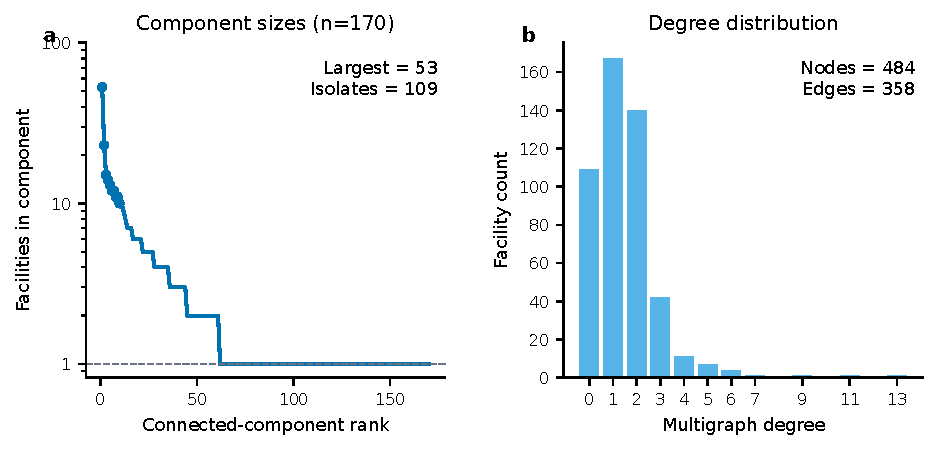
\includegraphics[width=\textwidth]{fig3_topology_quality.pdf}
  \caption{Geographic distribution and component structure of the selected candidate graph. Panel a uses released EPSG:4326 coordinates without a basemap or facility labels; blue branches belong to the 53-facility largest component, gray branches to other components, green points are connected facilities, and orange crosses are isolates. Panel b ranks all 170 components on a logarithmic scale. The graph contains 484 facilities, 358 candidate branches, and 109 isolates.}
  \label{fig:topology-quality}
\end{figure}

\FloatBarrier
\section{Technical Validation}

\subsection{Claim-bounded validation framework}

Validation is organized around five complementary evidence layers: machine-readable integrity, ledger and graph consistency, reconstruction sensitivity, OSM-derived public concordance, and electrical-readiness metadata. Table~\ref{tab:claim-bounded-validation} states what each layer evaluates and how the resulting evidence can be used. This framework places the scope of each result before the detailed tests, helping readers distinguish reproducibility and concordance evidence from questions that require an authoritative reference network.

No human-adjudicated or operator-supplied truth set was available for this release. The manuscript therefore reports measured consistency, sensitivity, concordance, and perturbation results rather than precision or recall estimates.

\begin{table}[!ht]
\centering
\small
\caption{Validation framework for the public-source data descriptor. Each layer contributes a defined form of reusable evidence.}
\label{tab:claim-bounded-validation}
\begin{tabular}{p{0.30\textwidth}p{0.31\textwidth}p{0.29\textwidth}}
\toprule
Validation layer & Evaluated property & Supported use \\
\midrule
Geometry, CRS, schema, and key checks & Machine readability and internal coherence & Reproducible loading and integration \\
Ledger and graph/table parity & Complete accounting under declared rules & Audit of retained and non-retained outcomes \\
216-setting sensitivity sweep & Dependence on reconstruction choices & Comparison of alternative configurations \\
OSM-derived public evidence & Public name and corridor concordance & Branch review and evidence prioritization \\
Electrical-readiness metadata & Availability and semantic status of required fields & Readiness filtering for downstream studies \\
\bottomrule
\end{tabular}
\end{table}
\FloatBarrier

\subsection{Internal validation}

The workflow applies fail-closed checks throughout acquisition, reconstruction, validation, and packaging. These checks include geometry-type and geometry-validity screening, coordinate-reference handling, endpoint completeness, facility-membership ambiguity, endpoint-cluster composition, mixed voltage or status conflicts, terminal-count classification, branch-key uniqueness, graph/table parity, schema coverage, manifest coverage, and checksum reconciliation.

Archive-level validation additionally checks that all 67 released files are documented, all manifest and checksum paths resolve, all 58 machine-readable paths have dictionary coverage, and the frozen headline counts agree with the core records. These results establish a consistent, independently checkable package for reuse.

\subsection{Structural validation}

Structural validation focuses on whether the reconstructed records satisfy the declared topology-building rules. Under the selected setting, the workflow converts 5,334 line features into 1,341 merged circuit candidates, of which 358 are retained and 983 are non-retained. The non-retained outcomes comprise 496 single-facility records, 216 isolated records, 104 tap or multi-terminal records, 101 self-loops, 61 ambiguous records, and five loop records for the current snapshot. Their preservation is itself a validation feature because it prevents silent loss of evidence about reconstruction uncertainty.

\subsection{Acquisition and projection stability}
\label{sec:projection-transition-audit}

The public acquisition procedure was repeated on 15 July 2026 through the E-REDES API. The source-input manifest records dataset identifiers, retrieval times, SHA-256 digests, byte sizes, and record counts for the retrieved CSV and GeoJSON inputs. This confirms execution of the documented acquisition route and provides a fingerprinted repeat-acquisition record for comparison with the deposited snapshot.

Projection stability was tested before freezing \dataset. For the 43,505 adjacent source-line segments, the legacy national-centre equirectangular implementation differed from spherical great-circle distances by 0.47\% at the median, 2.36\% at the 95th percentile, and 3.84\% at the maximum. The complete 216-configuration sweep was therefore rerun using ETRS89 / Portugal TM06 (EPSG:3763), and the final release adopts that result rather than retaining the legacy metric implementation.

The selected configuration remained node set B, a 100~m facility buffer, a 0.5~m endpoint snap threshold, and voltage-plus-status-aware merging. Both builds retained 358 branches, but one source-line group changed: 357 of 358 retained groups (99.72\%) preserved their facility endpoint pair, the ANTAS--PARANHOS branch from the legacy build was removed, and the SÃO JOÃO DE PONTE--SENHORA DO PORTO branch entered the final release. The corresponding release-local branch identifiers and source-line membership are recorded in \path{validation/projection\_release\_transition.csv}; the summary is in \path{validation/projection\_release\_transition\_summary.json}. The final EPSG:3763 build contains 1,341 circuit candidates, comprising 358 retained branches and 983 non-retained outcomes.

\subsection{Schema validation}

The release validates that required files, columns, and machine-readable summaries exist and remain aligned across the retained branch table, full ledger, GraphML, provenance, validation, and archive-control surfaces. The schema package distinguishes identifiers, observed and derived values, provenance metadata, validation variables, and explicit missing electrical fields.

For the frozen public-validation route, the internal validation export records 25 machine-readable checks across source geometry parsing, retained-branch completeness, ledger accounting, endpoint summaries, facility footprints, GraphML/table parity, sensitivity rows, and artifact hashes. All 25 checks pass for the released archive. Clean-room extraction validation reports no manifest, checksum, dictionary-coverage, or headline-count failures. The same export records 5,334 valid source geometries and zero invalid/dropped geometries; zero missing required retained-branch fields; zero missing required ledger fields; 358 retained branches; 983 non-retained outcomes; 1,341 ledger rows; 64,008 endpoint-index rows across six snap thresholds; and 216 sensitivity rows. Two detached worktrees of the annotated release tag independently rebuilt the archive from the same frozen derived inputs and produced the identical SHA-256 digest reported in the Data Record.

\subsection{Referential integrity}

Referential checks confirm that endpoint facility references, GraphML node and edge identifiers, branch-level validation records, source manifests, and manifest-linked artifact relationships resolve to valid upstream records. Graph and table views are checked for parity so that the GraphML, retained branch table, and selected facility set remain consistent with the documented isolate policy.

\subsection{Graph consistency}

The selected all-facility graph contains 484 facilities, 358 multiedges, 170 connected components, a largest component of size 53, 109 isolates, and 28 parallel edges. The edge-induced graph contains 375 incident facilities, while the all-facility GraphML additionally preserves selected isolates. This accounting distinction is stored explicitly so that users can reconcile graph artifacts with different isolate policies. Graph-level summaries validate the released artifact against its declared representation.

The GraphML/table parity check confirms that all 358 retained branch identifiers appear as GraphML edge identifiers, that no extra GraphML branch identifiers are present, and that every retained branch endpoint facility resolves to a GraphML node. The GraphML has 27 parallel facility pairs, 55 edge records participating in parallel pairs, and 28 extra parallel-edge records beyond one edge per facility pair. The missingness export also confirms that all retained-branch electrical fields \code{r}, \code{x}, \code{b}, thermal limits, transformer impedance, and tap settings remain explicitly marked as \status{MISSING\_NOT\_ESTIMATED}; these missing values are part of the release semantics rather than silent nulls.

\subsection{Sensitivity analysis}

Sensitivity analysis addresses whether the selected release point is stable under the declared reconstruction design space. The direct endpoint-to-substation baseline yields 51 merged edges and a six-node largest component, whereas the selected reconstruction yields 358 retained edges and a 53-node largest component for the current snapshot. These values quantify how the two workflows change retained yield and graph connectivity.

Across the 216-setting sweep, increasing the facility buffer from 100~m to 500~m at a 0.5~m endpoint snap threshold raises retained branches from 358 to 368 but also increases ambiguity from 61 to 89 and reduces the largest component from 53 to 27. At 50~m endpoint snapping, only three inter-facility circuits remain for each tested buffer. Figure~\ref{fig:sensitivity} shows these trade-offs and the selected operating point. The complete sweep makes parameter dependence visible and supports comparison of yield, ambiguity, and connectivity across plausible preprocessing choices.

\begin{figure}[t]
  \centering
  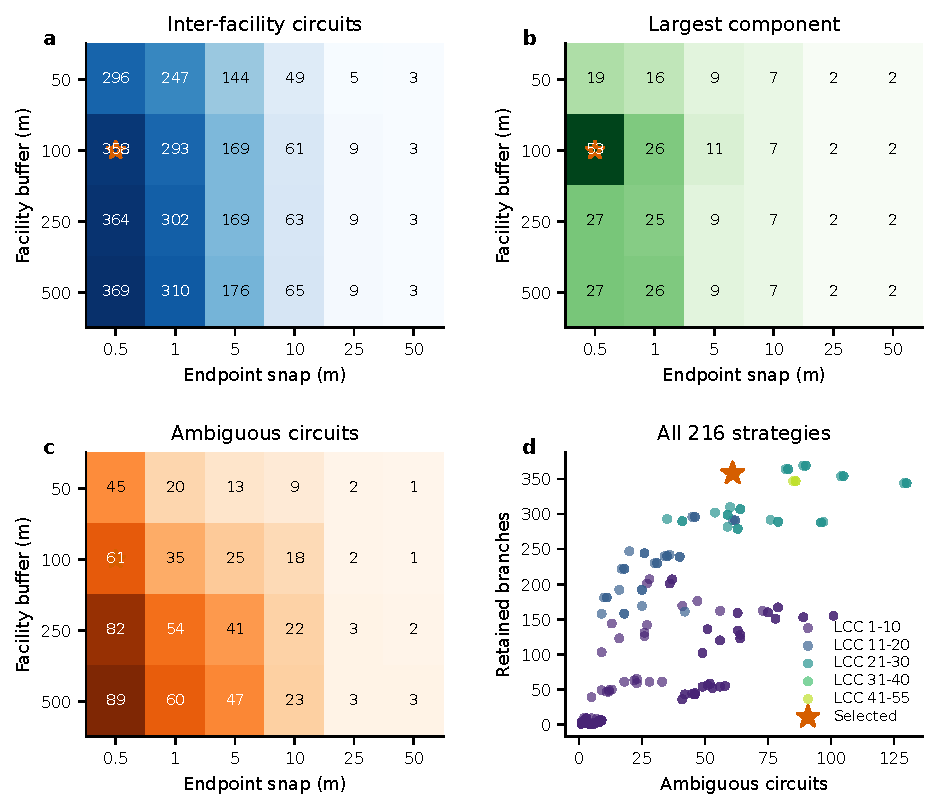
\includegraphics[width=\textwidth]{fig4_sensitivity_analysis.pdf}
  \caption{Sensitivity of retained-branch counts, ambiguity, and graph connectivity to facility buffers and endpoint snap thresholds. The marked operating point is the setting selected by the documented scoring rule.}
  \label{fig:sensitivity}
\end{figure}

\subsection{External triangulation}

The external triangulation workflow searches for OSM-derived branch-level evidence outside the selected reconstruction rule. OSM is the underlying public-evidence source; OpenInfraMap appears only as a visualization interface for the same OSM records and contributes no independent topology observations \cite{OSM2026,OpenInfraMap2026}. The matcher parses 60~kV OSM \code{power=line} and \code{power=cable} voltage, operator, name, reference, circuit, and geometry fields. A name score must be at least 0.8. Strong spatial evidence requires minimum distance no greater than 250~m, median branch-to-OSM distance no greater than 500~m, and branch or OSM coverage of at least 0.5 within 500~m; weak proximity is limited to 1,000~m. The operator-tag condition uses normalized user-contributed text containing \code{e redes} as one matching variable.

\begin{table}[t]
\centering
\small
\caption{OSM-derived public-evidence categories for the 358 retained candidate branches. The categories support branch-level review prioritization; machine category codes and matching variables remain in the deposited validation table.}
\label{tab:osm-triangulation}
% Generated from PT60-Candidate v1.0.0; do not edit by hand.
\begin{tabular}{p{0.46\textwidth}rp{0.32\textwidth}}
\toprule
Evidence category & Branches & Interpretation \\
\midrule
\status{OSM\_NAME\_OPERATOR\_STRONG} & 183 & Endpoint names appear in a 60~kV E-REDES-labelled OSM record. \\
\status{OSM\_GEOMETRY\_OPERATOR\_STRONG} & 64 & Candidate corridor is close to a 60~kV E-REDES-labelled OSM corridor. \\
\status{OSM\_PARTIAL\_NAME\_NEARBY} & 56 & One endpoint name appears and a nearby 60~kV corridor is present. \\
\status{OSM\_GEOMETRY\_MEDIUM} & 48 & Candidate overlaps a 60~kV public corridor without strong name evidence. \\
\status{OSM\_NEARBY\_WEAK} & 7 & A nearby 60~kV public feature is present, but evidence is incomplete. \\
\status{NO\_EXTERNAL\_OSM\_MATCH} & 0 & No retained branch falls in this class for the documented snapshot. \\
\bottomrule
\end{tabular}

\end{table}

Table~\ref{tab:osm-triangulation} gives the category counts. Among 5,551 Portuguese 60~kV OSM ways, all 358 retained branches receive a non-empty evidence category: 245 strong, 106 medium, and seven weak. The five displayed categories are mutually exclusive priority labels. The spatial negative control uses a separate cross-category corridor indicator, so its baseline is not obtained by summing whole categories in Table~\ref{tab:osm-triangulation}. A provenance-risk audit of 2,313 historical versions for 270 matched OSM ways classifies 266 branches as lower risk, 87 as unknown independence, and five as possibly same-source. These audit variables allow users to filter or prioritize concordance evidence according to source-independence risk. The archive provides sanitized evidence tables while omitting user identifiers, changesets, histories, and raw caches.

\subsection{Matcher selectivity controls}

Two deterministic controls test matcher selectivity on all 358 branches. With geometry and branch attributes fixed, a length-stratified cyclic shift of endpoint-name pairs (seed 20260714) reduces strong name evidence from 182 to 9 branches (95.1\%). For the spatial control, corridor evidence is defined independently of the priority categories as \code{min\_distance\_m}$\leq250$~m together with either \code{branch\_coverage\_500m}$\geq0.5$ or \code{osm\_coverage\_500m}$\geq0.5$. In the undisplaced matches, this criterion is met by all 63 geometry-operator-strong records, all 50 geometry-medium records, and 177 of the 182 name-operator-strong records, giving $63+50+177=290$ branches; the partial-name and weak categories contribute zero. With names and attributes fixed, translation by $+1.75^\circ$ longitude and $+0.85^\circ$ latitude leaves all geometries valid but reduces this corridor-evidence count from 290 to 1 branch (99.7\%).

Together, the two perturbation tests show that the matcher responds selectively to endpoint-name and spatial-corridor information. Their interpretation follows the validation framework in Table~\ref{tab:claim-bounded-validation}.

\FloatBarrier
\section{Usage Notes}

\subsection{Intended uses}

The core release is intended for topology-reconstruction studies, geospatial data integration, provenance-aware network analysis, uncertainty analysis, dataset-engineering experiments, and development of downstream graph or tabular interfaces that preserve release semantics. The retained branch table and circuit-classification ledger should be used together whenever a study depends on understanding what was retained, what remained non-retained, and why.

\subsection{Non-intended uses}

The release is not intended for operational switching studies, protection analysis, security assessment, contingency analysis, congestion forecasting, infrastructure-targeting applications, emergency operations, asset-condition assessment, commercial network-capacity claims, regulatory network-capacity claims, or claims about the actual Portuguese grid. The candidate topology should not be described as operator-validated, and the optional diagnostic electrical and learning layers should not be described as measured system behavior.

\subsection{Reading provenance and semantic status fields}

Users should read semantic status fields before aggregating or modeling the records. Observed, derived, inferred, source-backed, scenario-assumed, benchmark-only, proxy, and missing fields represent distinct evidence types. Studies that require source-backed physical parameters or operator-confirmed connectivity should filter the release accordingly and should not treat inferred or scenario-derived fields as interchangeable with observations.

\subsection{How to use GraphML}

The GraphML is the most direct representation of the released candidate multigraph for graph analysis. It preserves the selected all-facility node set, including isolates, and therefore aligns with the documented component and degree summaries. Users comparing the GraphML with edge-induced views should account for the explicit isolate policy. Parallel edges are part of the released graph structure and should not be collapsed without documenting the transformation.

\subsection{How to use CSV records}

The retained candidate branch CSV is the preferred branch-level topology table. The circuit-classification ledger should be consulted whenever a downstream workflow depends on failure modes, ambiguity, or alternative selection rules. Validation CSV and JSON records document evidence categories, matcher controls, independence-risk categories, missingness, and archive-validation relationships. The six recommended joins in \code{schema/join\_relationships.csv} should be used in preference to name-based joins.

\subsection{Limitations}

The release has three main limitations. First, it is a candidate topology derived from public E-REDES records rather than an operator-confirmed network model. Second, external triangulation provides public-source concordance categories rather than truth labels: precision is not independently estimated, and national or real-network recall cannot be estimated from the available records. Third, electrical parameters, transformer details, operating controls, and injections are incomplete or absent, so the release is not AC power-flow or OPF ready.

\section*{Data Availability}

\dataset{} is prepared for deposition under the reserved figshare DOI \url{https://doi.org/10.6084/m9.figshare.32984021}. The deposited archive has SHA-256 \hashvalue{328e64adcfc6c7210ed9558793a14fdb661e5e3bab741f1d275a89e5593d1447}. It contains the core topology, full circuit ledger, GraphML, sensitivity sweep, provenance, validation, machine-readable schemas, a field-level data dictionary, licensing, attribution, manifest, and checksum records described in the Data Record. Raw source downloads and optional diagnostic/interface artifacts are excluded as documented in \path{excluded\_artifacts.json}. E-REDES-derived records remain subject to the attribution and indication-of-modification terms documented in \path{DATA\_LICENSE.md} and \path{ATTRIBUTION.md}; the software licence does not replace those data terms.

\section*{Code Availability}

The source code is publicly available at \url{https://github.com/MingLeiZhou/PortugueseOPD}. The released source is preserved by an annotated release tag at commit \code{93c861c}; two detached clean worktrees of that tag produced byte-identical archives from the frozen derived inputs. The reference environment uses Python~3.12.9 and the versioned \path{requirements.txt}; the software is MIT licensed. No separate software DOI is claimed. The acquisition code retrieves the source inputs through the public E-REDES API using widget API keys discovered from the official RND page. The acquisition procedure is repeatable at the reported access date, while exact reconstruction of the deposited archive is anchored by its recorded inputs, manifests, checksums, and tagged build.

\begin{thebibliography}{12}

\bibitem{Medjroubi2017}
Medjroubi, W., Müller, U. P., Scharf, M., Matke, C. \& Kleinhans, D. Open data in power grid modelling: new approaches towards transparent grid models. \emph{Energy Rep.} \textbf{3}, 14--21 (2017). \doi{10.1016/j.egyr.2016.12.001}

\bibitem{Horsch2018}
Hörsch, J., Hofmann, F., Schlachtberger, D. \& Brown, T. PyPSA-Eur: an open optimisation model of the European transmission system. \emph{Energy Strategy Rev.} \textbf{22}, 207--215 (2018). \doi{10.1016/j.esr.2018.08.012}

\bibitem{Wiese2019}
Wiese, F. \emph{et al.} Open Power System Data--frictionless data for electricity system modelling. \emph{Appl. Energy} \textbf{236}, 401--409 (2019). \doi{10.1016/j.apenergy.2018.11.097}

\bibitem{Xiong2025}
Xiong, B., Fioriti, D., Neumann, F., Riepin, I. \& Brown, T. Modelling the high-voltage grid using open data for Europe and beyond. \emph{Sci. Data} \textbf{12}, 277 (2025). \doi{10.1038/s41597-025-04550-7}

\bibitem{Rivera2019}
Rivera, J., Nasirifard, P., Leimhofer, J. \& Jacobsen, H.-A. Automatic generation of real power transmission grid models from crowdsourced data. \emph{IEEE Trans. Smart Grid} \textbf{10}, 5436--5448 (2019). \doi{10.1109/TSG.2018.2882840}

\bibitem{Haklay2008}
Haklay, M. \& Weber, P. OpenStreetMap: user-generated street maps. \emph{IEEE Pervasive Comput.} \textbf{7}, 12--18 (2008). \doi{10.1109/MPRV.2008.80}

\bibitem{Wilkinson2016}
Wilkinson, M. D. \emph{et al.} The FAIR Guiding Principles for scientific data management and stewardship. \emph{Sci. Data} \textbf{3}, 160018 (2016). \doi{10.1038/sdata.2016.18}

\bibitem{Gebru2021}
Gebru, T. \emph{et al.} Datasheets for datasets. \emph{Commun. ACM} \textbf{64}, 86--92 (2021). \doi{10.1145/3458723}

\bibitem{EREDESOpenData2026}
E-REDES. E-REDES Open Data Portal. \url{https://e-redes.opendatasoft.com/pages/homepage/} (accessed 13 July 2026).

\bibitem{OpendatasoftExploreAPI2026}
Opendatasoft. Explore API v2.1 reference: geometry export \code{epsg} parameter. \url{https://help.opendatasoft.com/apis/ods-explore-v2/} (accessed 15 July 2026).

\bibitem{PT60Candidate2026}
PortugueseOPD contributors. PT60-Candidate: a provenance-tracked candidate dataset for Portuguese 60 kV topology reconstruction. figshare \doi{10.6084/m9.figshare.32984021} (2026).

\bibitem{OSM2026}
OpenStreetMap contributors. OpenStreetMap. \url{https://www.openstreetmap.org/} (accessed 13 July 2026).

\bibitem{OpenInfraMap2026}
OpenInfraMap contributors. OpenInfraMap. \url{https://www.openinframap.org/} (accessed 13 July 2026).

\end{thebibliography}

\section*{Author Contributions}

The author-responsibility statement will be completed when the final author list is supplied and before submission.

\section*{Competing Interests}

The final competing-interests declaration will be supplied before submission.

\section*{Acknowledgements}

Acknowledgements, if applicable, will be finalized before submission.

\section*{Funding}

The funding statement will be finalized before submission.

\end{document}
